% !TEX root = ../main.tex
%

\chapter{自動微分}

自動微分 (automatic differentiation) では,
関数 $\bm{f} : \setR^m \to \setR^n$ の
関数値 $\bm{f}(\bm{x})$ を求めるために必要な演算をもとに
Jacobian $\partial \bm{f} / \partial \bm{x}$ を自動で算出する
\cite{Kubota1998}.

自動微分では,微分/偏微分における合成関数の微分公式
\begin{equation}
    \frac{\partial \bm{f}(\bm{g}(\bm{x}))}{\partial \bm{x}}
    = \frac{\partial \bm{f}(\bm{g}(\bm{x}))}{\partial \bm{g}(\bm{x})}
    \frac{\partial \bm{g}(\bm{x})}{\partial \bm{x}}
    \label{eq:differentiation_auto-diff_chain-rule}
\end{equation}
を利用する.
右辺値を右側から計算していくか,左側から計算していくかにより,
それぞれ前進型自動微分 (forward-mode automatic differentiation),
後退型自動微分 (backward-mode automatic differentiation) と呼び分けられる.

\section{前進型自動微分}

前進型自動微分では,
式 \eqref{eq:differentiation_auto-diff_chain-rule} における
$\bm{g}(\bm{x})$ の Jacobian が分かっている状態から
$\bm{f}(\bm{g}(\bm{x}))$ の Jacobian を算出する
\cite{Kubota1998}.

例えば,$\sin(\cos(x))$ を計算する場合,次のようにする.

\begin{enumerate}
    \item 変数値 $x$ と微分係数 $1$ から計算を始める.
    \item 中間的な関数値 $y = \cos{x}$ を算出するのに併せて微分係数 $y' = -\sin{x}$ を算出する.
    \item 関数値 $z = \sin{y}$ を算出するのに併せて微分係数 $z' = y' \cos{y}$ を算出する.
\end{enumerate}

この仕組みでは,
各変数に対して微分係数用の領域を用意して計算を進めていく.

\section{後退型自動微分}

前進型自動微分では,
式 \eqref{eq:differentiation_auto-diff_chain-rule} における
$\bm{f}(\bm{y})$ の Jacobian が分かっている状態から
$\bm{f}(\bm{g}(\bm{x}))$ の Jacobian を算出する
\cite{Kubota1998}.

例えば,$\sin(\cos(x))$ を計算する場合,次のようにする.

\begin{enumerate}
    \item 中間的な関数値 $y = \cos{x}$ を算出し,$\cos$ の計算をしたことを記録する.
    \item 関数値 $z = \sin{y}$ を算出し,$\sin$ の計算をしたことを記録する.
    \item 微分係数 $1$ から計算を始め,$1 \cdot dz/dy = \cos{y}$ を計算する.
    \item $1 \cdot dz/dy \cdot dy/dx = \cos{y} \cdot (-\sin{x})$ を計算する.
\end{enumerate}

\begin{figure}[tp]
    \centering
    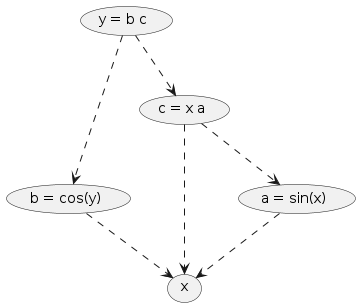
\includegraphics[width=0.5\linewidth]{differentiation/auto-diff-backward/example-nodes.png}
    \caption{後退型自動微分における計算グラフの例}
    \label{fig:differentiation_auto-diff_backward-nodes-example}
\end{figure}

\begin{algorithm}[tp]
    \caption{後退型自動微分における微分係数の計算}
    \label{alg:differentiation_auto-diff_backward-derivative-calculation}
    \begin{algorithmic}
        \Procedure{BackwardModeAutomaticDifferentiation}{グラフ, 微分の対象となるノード}
        \State $V, r = \text{ListRequiredNodes}(\text{グラフ, 微分の対象となるノード})$
        \Comment Algorithm \ref{alg:differentiation_auto-diff_backward-derivative-calculation-2}
        \ForAll{$V$ の要素 $v$}
        \State $d(v) \gets 0$ \Comment 微分係数
        \State $a(v) \gets 0$ \Comment 微分係数の加算を行った回数
        \EndFor
        \State $d(\text{微分の対象となるノード}) \gets 1$
        \State 空の処理待ちのキューを用意する.
        \State 処理待ちのキューに微分の対象となるノードを追加する.
        \While{処理待ちのキューに要素がある}
        \State 処理待ちのキューから要素を取り出し,$v$ とする.
        \ForAll{$v$ が参照しているノード $w$}
        \State $v$ を $w$ で偏微分した係数 $f$ を計算する.
        \State $d(w) \gets d(w) + f d(v)$
        \State $a(w) \gets a(w) + 1$
        \If{$a(w) = r(w)$}
        \State $w$ を処理待ちのキューに追加する.
        \EndIf
        \EndFor
        \EndWhile
        \EndProcedure
    \end{algorithmic}
\end{algorithm}
\begin{algorithm}[tp]
    \caption{後退型自動微分における微分係数の計算におけるサブルーチン ListRequiredNodes}
    \label{alg:differentiation_auto-diff_backward-derivative-calculation-2}
    \begin{algorithmic}
        \Procedure{ListRequiredNodes}{グラフ, 微分の対象となるノード}
        \State $V \gets \{\text{微分の対象となるノード}\}$ \Comment 必要なノードの一覧
        \State $r(\text{微分の対象となるノード}) \gets 0$ \Comment ノードが参照されている回数
        \State 空の処理待ちのキューを用意する.
        \State 処理待ちのキューに微分の対象となるノードを追加する.
        \While{処理待ちのキューに要素がある}
        \State 処理待ちのキューから要素を取り出し,$v$ とする.
        \ForAll{$v$ が参照しているノード $w$}
        \If{$r(w)$ が定義されている}
        \State $r(w) \gets r(w) + 1$
        \Else
        \State $r(w) \gets 1$
        \EndIf
        \If{$w$ が $V$ にない}
        \State $V \gets V + \{w\}$
        \State $w$ を処理待ちのキューに追加する.
        \EndIf
        \EndFor
        \EndWhile
        \State \Return $V$, $r$
        \EndProcedure
    \end{algorithmic}
\end{algorithm}

後退型自動微分においては,
計算時とは逆順に微分係数の計算を行う必要がある.
そこで,
図 \ref{fig:differentiation_auto-diff_backward-nodes-example}
のような計算グラフと呼ばれるものを考える\cite{Kubota1998}.
図 \ref{fig:differentiation_auto-diff_backward-nodes-example}
の中で上の方にあるノードから順に微分係数の計算を進めていく方法としては,
例えば
Algorithm \ref{alg:differentiation_auto-diff_backward-derivative-calculation}
が考えられる
\footnote{文献 \cite{Kubota1998} には実装に使用できるレベルのアルゴリズムが見当たらなかったため,%
    トポロジカルソートをベースに考案した.}.
